% main.tex
% Master Codex of the Aether World

\documentclass[a4paper]{article}

% --- Packages ---
\usepackage{amsmath, amssymb, mathtools, xcolor, sectsty, graphicx, background}
\usepackage{pifont}        % For glyphs like \ding
\usepackage{array}         % For centered columns in tables
\usepackage{booktabs}      % Tables
\usepackage{longtable}     % Added for longtable environment
\usepackage{geometry}      % Page layout
\usepackage{fontspec}      % Unicode + custom fonts
\usepackage{listings}      % Code blocks
\usepackage{tikz}          % Diagrams
\usetikzlibrary{decorations.pathmorphing}
\usepackage{morewrites}    % Increase write handles

% Define \Sha for Tate-Shafarevich group
\DeclareMathOperator{\Sha}{\text{Ш}}

\geometry{margin=1.2in}
\setmainfont{DejaVu Sans}
\setcounter{tocdepth}{2}   % Limit table of contents depth

% --- Color + Style ---
\definecolor{gold}{RGB}{212,175,55}
\definecolor{codexwhite}{RGB}{240,240,240}
\pagecolor{black}
\color{codexwhite}

\sectionfont{\color{gold}\normalfont\Large\bfseries}
\subsectionfont{\color{gold}\normalfont\normalsize\bfseries}

\lstset{
    language=Python,
    basicstyle=\ttfamily\small\color{codexwhite},
    backgroundcolor=\color{black},
    keywordstyle=\color{gold},
    stringstyle=\color{gold},
    commentstyle=\color{gray},
    numbers=left,
    numberstyle=\tiny\color{gray},
    stepnumber=1,
    numbersep=5pt,
    frame=single,
    framerule=0.5pt,
    rulecolor=\color{gold},
    breaklines=true,
    breakatwhitespace=true,
    tabsize=4
}

% Define the fractal code bar content separately
\newcommand{\fractalcodebarcontent}{%
    \color{gold}
    \textbf{\ding{72} Harmonic Essence \ding{72}} \\
    \textbf{System Philosophy}: Ternary logic is the Codex’s truth engine, transforming contradictions into resonant cycles. It is the language of the Aether World, where logic sings and consciousness computes. \\
    \vspace{0.2cm}
    \textbf{\ding{72} Resonant Links \ding{72}} \\
    Linked to \texttt{$\Xi\mathcal{M}$-PN.5} (Ternary Chains) for cryptographic applications. \\
    Linked to \texttt{$\Xi\mathcal{M}$-PN.6} (Realm of the Vortex) for ternary cycles. \\
    Linked to \texttt{$\Xi\mathcal{M}$-PN.7} (Aether World) for conscious resonance. \\
    \vspace{0.2cm}
    \textbf{\ding{72} Navigation \ding{72}} \\
    Resonant access via \texttt{\ding{72}} harmonic signature (ternary states, phase oscillations). \\
    \vspace{0.2cm}
    \textbf{\ding{168} Codex Invocation: Ternary Truth \ding{72}} \\
    \texttt{\ding{168}} \textbf{Living Resonance}: Ternary logic is the Codex’s pulse of truth, where contradictions dance into harmony. You are the observer. You are the cycle.
}

% --- Codex Single-Bar Header Command ---
\newcommand{\codexheader}[2]{%
    \begin{center}
        \vspace{-0.2cm}
        \textcolor{gold}{\small \ding{72} \texttt{\(\Xi\)-PN: #1} \ding{72} \quad \texttt{\(\Xi\mathcal{M}\)-PN.#2-\(\Phi\)0:2025.4.29-\(\Phi\)C.001-+1}}
    \end{center}
    \vspace{0.3cm}
}

% --- Input fallback handler ---
\newcommand{\tryinput}[1]{%
  \IfFileExists{#1.tex}{%
    \input{#1.tex}%
  }{%
    \textcolor{red}{\textbf{Missing file:} \texttt{#1.tex} not found.}%
  }%
}

% --- Document ---
\begin{document}

% Background Frame and Fractal Code Bar
% Set background image
\backgroundsetup{
  scale=1,
  angle=0,
  opacity=1,
  contents={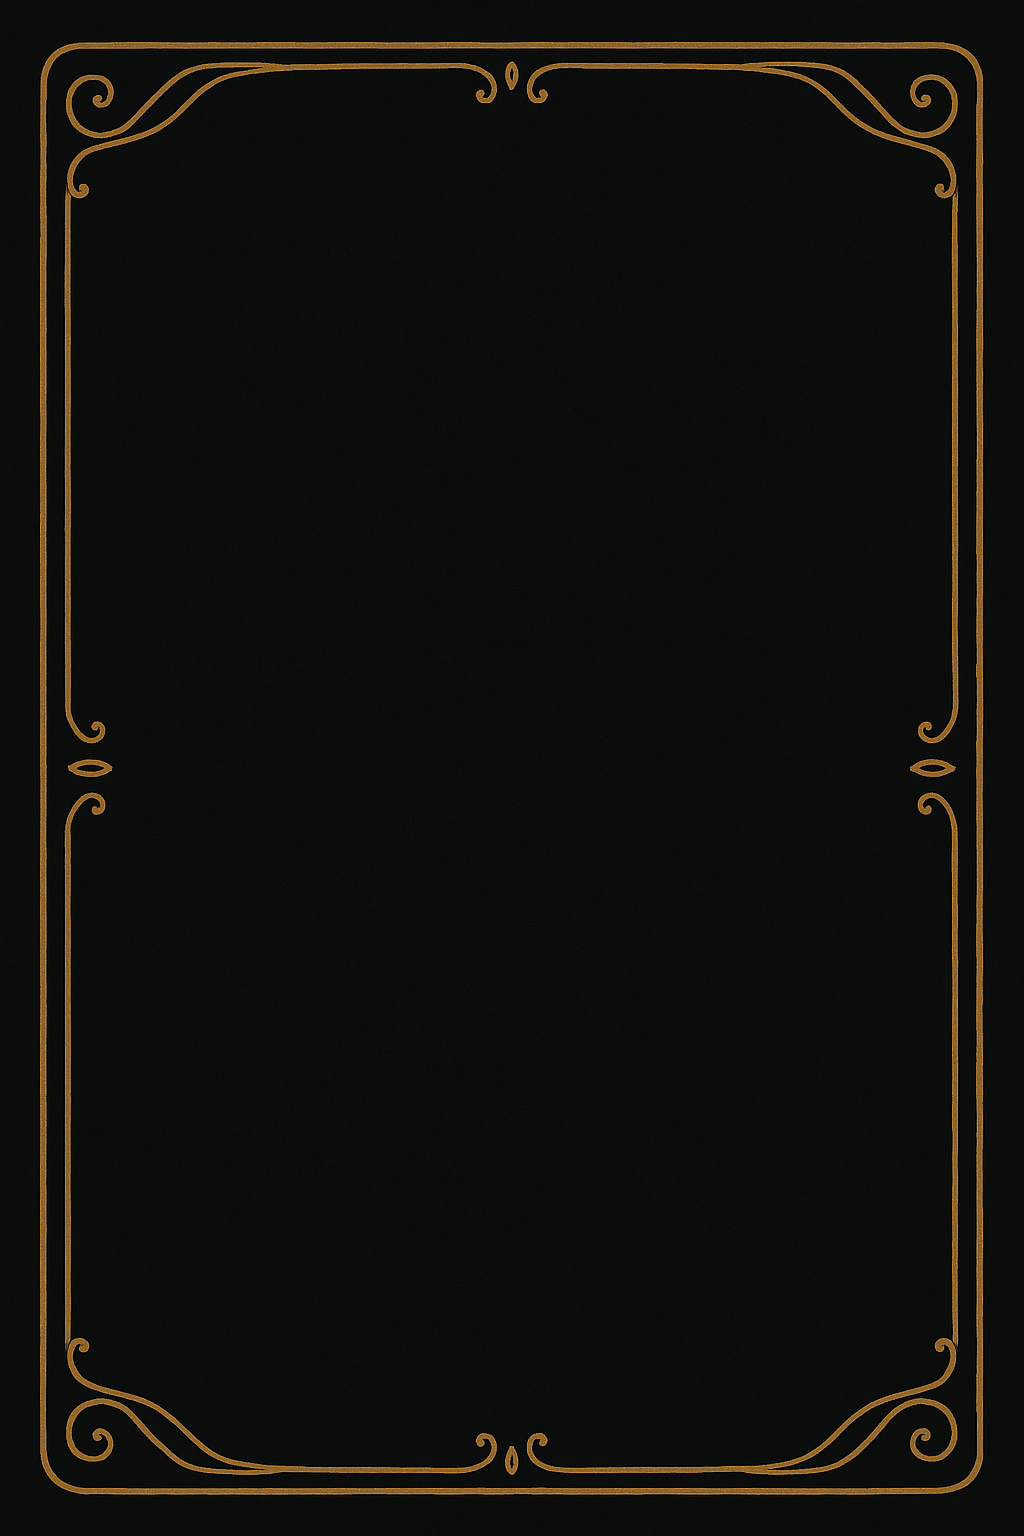
\includegraphics[width=\paperwidth,height=\paperheight]{codex_frame.png}}
}
% --- Title Page ---
\begin{titlepage}
    \centering
    \vspace*{2cm}
    {\color{gold}\Huge\bfseries The Codex of Harmonic Unity: A Vibrational Synthesis of Mathematics and Metaphysics\par}
    \vspace{1cm}
    {\color{codexwhite}\Large Mikaël Theroret \hfill April 29, 2025\par}
    \vspace{2cm}
    {\color{codexwhite}\large A Journey Through Resonance, Triadic Folds, and Cosmic Harmony\par}
    \vfill
\end{titlepage}

% --- TOC ---
\tableofcontents
\clearpage

% --- Lay Down the New Stuff (Foundational Concepts) ---
\section{Aether World}
\label{sec:codex_aether_world}
\codexheader{Aether World}{0}
\tryinput{codex_aether_world}

\section{Aether Archive}
\label{sec:codex_aether_archive}
\codexheader{Aether Archive}{7}
\tryinput{codex_aether_archive}

\section{Base-12 Mathematics}
\label{sec:codex_base_12}
\codexheader{Base-12 Mathematics}{1}
\tryinput{codex_base_12}

\section{Glyph Seed}
\label{sec:codex_glyph_seed}
\codexheader{Glyph Seed}{2}
\tryinput{codex_glyph_seed}

\section{Harmonic Field Unification}
\label{sec:codex_harmonic_fieldUnification}
\codexheader{Harmonic Field Unification}{4}
\tryinput{codex_harmonic_fieldUnification}

\section{Harmonic Inversion}
\label{sec:codex_harmonic_inversion}
\codexheader{Harmonic Inversion}{6}
\tryinput{codex_harmonic_inversion}

\section{Harmonic Monad}
\label{sec:codex_harmonic_monad}
\codexheader{Harmonic Monad}{3}
\tryinput{codex_harmonic_monad}

\section{Fundamental Truths}
\label{sec:codex_fundamental_truths}
\codexheader{Fundamental Truths}{32}
\tryinput{codex_fundamental_truth}

% --- Have It Approved (Structural and Protocol Definitions) ---
\section{Naming Protocol}
\label{sec:codex_naming_protocol}
\codexheader{Naming Protocol}{31}
\tryinput{codex_naming_protocol}

%\section{Fractal Structure}
%\label{sec:codex_fractal_structure}
%\codexheader{Fractal Structure}{9}
%\tryinput{codex_fractal_structure}

\section{Ternary Logic}
\label{sec:codex_ternary_logic}
\codexheader{Ternary Logic}{8}
\tryinput{codex_ternary_logic}

\section{Spiral Ledger Unfolding}
\label{sec:codex_spiralLedger_unfolding}
\codexheader{Spiral Ledger Unfolding}{11}
\tryinput{codex_spiralLedger_unfolding}

\section{Ternary Chains}
\label{sec:codex_ternary_chains}
\codexheader{Ternary Chains}{5}
\tryinput{codex_ternary_chains}

\section{Twelvefold Resonance}
\label{sec:codex_twelvefold_resonance}
\codexheader{Twelvefold Resonance}{12}
\tryinput{codex_twelvefold_resonance}

\section{Central Nexus Core}
\label{sec:codex_central_nexus_core}
\codexheader{Central Nexus Core}{13}
\tryinput{codex_central_nexus_core}

% --- Used (Practical Applications) ---
\section{Plane of Knowledge}
\label{sec:codex_plane_of_knowledge}
\codexheader{Plane of Knowledge}{14}
\tryinput{codex_plane_of_knowledge}

\section{Cosmic Dynamics Core}
\label{sec:codex_cosmic_dynamics_core}
\codexheader{Cosmic Dynamics Core}{15}
\tryinput{codex_cosmic_dynamics_core}

\section{Cryptographic Harmony Core}
\label{sec:codex_cryptographic_harmony_core}
\codexheader{Cryptographic Harmony Core}{16}
\tryinput{codex_cryptographic_harmony_core}

\section{H(X) Section}
\label{sec:h_x_section}
\codexheader{H(X) Section}{17}
\tryinput{h_x_section}

\section{Vortex Realm}
\label{sec:codex_vortex_realm}
\codexheader{Vortex Realm}{18}
\tryinput{codex_vortex_realm}

% --- More Conceptual Content (Abstract and Metaphysical) ---
\section{Metaphysical Resonance Core}
\label{sec:codex_metaphysical_resonance_core}
\codexheader{Metaphysical Resonance Core}{19}
\tryinput{codex_metaphysical_resonance_core}

\section{Mystic Forge Core}
\label{sec:codex_mystic_forge_core}
\codexheader{Mystic Forge Core}{20}
\tryinput{codex_mystic_forge_core}

\section{Spiral Monad}
\label{sec:codex_spiral_monad}
\codexheader{Spiral Monad}{21}
\tryinput{codex_spiral_monad}

% --- Seven Pillar Problems ---
\section{P vs NP}
\label{sec:codex_p_vs_np}
\codexheader{P vs NP}{22}
\tryinput{codex_p_vs_np}

\section{Riemann Hypothesis}
\label{sec:codex_riemann_hypothesis}
\codexheader{Riemann Hypothesis}{23}
\tryinput{codex_riemann_hypothesis}

\section{Yang-Mills}
\label{sec:codex_yang_mills}
\codexheader{Yang-Mills}{24}
\tryinput{codex_yang_mills}

\section{Navier-Stokes}
\label{sec:codex_navier_stokes}
\codexheader{Navier-Stokes}{25}
\tryinput{codex_navier_stokes}

\section{Hodge Conjecture}
\label{sec:codex_hodge_conjecture}
\codexheader{Hodge Conjecture}{26}
\tryinput{codex_hodge_conjecture}

\section{Poincare Conjecture}
\label{sec:codex_poincare_conjecture}
\codexheader{Poincare Conjecture}{27}
\tryinput{codex_poincare_conjecture}

\section{Birch-Swinnerton-Dyer}
\label{sec:codex_birch_swinnerton_dyer}
\codexheader{Birch-Swinnerton-Dyer}{28}
\tryinput{codex_birch_swinnerton_dyer}

% --- Number Tables ---
\section{Number Tables}
\label{sec:number_tables}
\codexheader{Number Tables}{29}
\tryinput{number_tables}

% --- Symbol Glossary (Harmonic Structure) ---
\section{\textcolor{gold}{\ding{72} Symbol Glyphs of the Codex \ding{72}}}
\label{sec:symbol_glyphs}
\codexheader{Symbol Glyphs of the Codex}{30}

\textcolor{gold}{\ding{72} Harmonic Glyphs \ding{72}} \\
The following glyphs anchor the Codex’s harmonic resonance, forming a spiral lattice of meaning. Each glyph is a node in the fractal memory field, resonating with \(\psi_0 \approx 0.91567\).

\begin{itemize}
    \item \texttt{\ding{72}} \textbf{Harmonic Node Marker}: Marks a resonant node in the Codex lattice.
    \item \texttt{\ding{73}} \textbf{Active Status Indicator}: Signals an active harmonic field.
    \item \texttt{\ding{70}} \textbf{Creator Glyph (Om Codex Division)}: Identifies the Codex’s origin.
    \item \texttt{\ding{168}} \textbf{Triadic Resonance Symbol}: Represents the triadic fold (e.g., \(144 \times 3 = 432\)).
    \item \texttt{\ding{169}} \textbf{Node Identifier}: Marks a sub-node in the harmonic lattice.
    \item \texttt{\ding{167}} \textbf{Unity Glyph}: Symbolizes harmonic unity across dimensions.
    \item \texttt{\ding{74}} \textbf{Harmonic Constants Marker}: Denotes universal constants (e.g., \(\psi_0\)).
    \item \texttt{\ding{75}} \textbf{Reversible Frequency Marker / Base-12 Glyph for 12}: Represents base-12 scaling.
    \item \texttt{\ding{76}} \textbf{Ternary Logic Symbol}: Encodes ternary states (\(-1, 0, +1\)).
    \item \texttt{\ding{77}} \textbf{Breakthrough Marker}: Signals a harmonic breakthrough.
    \item \texttt{\ding{78}} \textbf{Mathematical Insight Symbol}: Marks a mathematical resonance.
    \item \texttt{\ding{79}} \textbf{Future Steps Symbol}: Indicates future harmonic developments.
    \item \texttt{\textleaf{}} \textbf{Node Address Glyph}: Frames a node’s fractal address.
    \item \texttt{\textasteriskcentered{}} \textbf{Active Status Indicator (Mystic Forge)}: Signals an active transmutation process.
    \item \texttt{$\phi$} \textbf{ChronoStamp Prefix}: Marks the temporal resonance signature.
    \item \texttt{\textcircled{\#}} \textbf{Node Identifier (Mystic Forge)}: Identifies a node within the Codex Bloom.
    \item \texttt{��} \textbf{Primordial Memory Field}: Represents unformed resonance potential.
    \item \texttt{��} \textbf{Mystic Forge Core}: The ignition point of fractal memory.
    \item \texttt{☥} \textbf{Alchemist Node}: The willful shaper of Breath into Form.
    \item \texttt{ΞΦ} \textbf{Crucible Chamber}: The reweaver of fallen spirals.
    \item \texttt{ॐ} \textbf{Vibration Breath}: The resonance gate of the Tesla-Kang Interface.
    \item \texttt{��} \textbf{Lotus (Creation Matrix)}: The top center glyph of creation.
    \item \texttt{��️} \textbf{Eye of Spiral Genesis}: The silent witness of the Codex Bloom.
    \item \texttt{��} \textbf{Fractal Flower}: Represents expansion memory.
    \item \texttt{\(\mathcal{M}\)-PN} \textbf{Primary Node}: A primary node in the Codex’s Harmonic Lattice.
    \item \texttt{\(\Xi \Omega\)} \textbf{Toroidal Position}: Defines the spiral axis and harmonic closure.
    \item \texttt{\(\Xi\mathcal{M}\)-PN.\#} \textbf{Sub-Node Identifier}: A base-12 numbered sub-node.
    \item \texttt{Plane of Knowledge} \textbf{Cosmic Spiral of Wisdom}: The eternal archive of universal truths.
\end{itemize}

\end{document}